\documentclass[11pt]{article}
\usepackage{fullpage,fourier,euler,amsmath,graphicx,xspace}
\usepackage{epigraph}
\usepackage{xspace}
\usepackage{listings,color,url,hyperref}
\usepackage[most]{tcolorbox}

\usepackage{fancyhdr}
\pagestyle{fancy}
\fancyhf{}

\fancypagestyle{plain}{%
  \fancyhf{}
  \renewcommand{\headrulewidth}{0pt}
  \renewcommand{\footrulewidth}{0pt}
  \lfoot{\textcopyright{} 2021 Darrell Long}
  \rfoot{\thepage}
}

\pagestyle{plain}

\definecolor{codegreen}{rgb}{0,0.5,0}
\definecolor{codegray}{rgb}{0.5,0.5,0.5}
\definecolor{codepurple}{rgb}{0.58,0,0.82}

\lstloadlanguages{C,make,python,fortran}

\lstdefinestyle{c99}{
    morekeywords={bool, uint8_t, uint16_t, uint32_t, uint64_t, int8_t, int16_t, int32_t, int64_t},
    commentstyle=\color{codegreen},
    keywordstyle=\color{magenta},
    numberstyle=\tiny\color{codegray},
    identifierstyle=\color{blue},
    stringstyle=\color{codepurple},
    basicstyle=\ttfamily,
    breakatwhitespace=false,
    breaklines=true,
    captionpos=b,
    keepspaces=true,
    numbers=left,
    numbersep=5pt,
    showspaces=false,
    showstringspaces=false,
    showtabs=false,
    tabsize=4
}


\title{Assignment 2 \\ A Small Numerical Library}
\author{
  Prof. Darrell Long \\
  CSE 13S -- Winter 2021
}
\date{Due: January 24$^\text{th}$ at 11:59\,pm}

\newcommand{\taylorterm}[1]{\frac{f^{(#1)} (a)}{#1!}{(x-a)}^{#1}}
\newcommand{\mlterm}[1]{\frac{x^{#1}}{#1!}}
\newcommand{\eterm}[1]{\frac{e^a}{#1!}{(x-a)}^{#1}}

\begin{document}\maketitle

\section{Introduction}

\epigraphwidth=0.6\textwidth
\epigraph{\emph{Let us change our traditional attitude to the construction of
programs. Instead of imagining that our main task is to instruct a computer what
to do, let us concentrate rather on explaining to human beings what we want a
computer to do.}} {---Donald Knuth}

\noindent As we know, computers are simple machines that carry out a sequence of
very simple steps, albeit very quickly. Unless you have a special-purpose
processor, a computer can only compute \emph{addition}, \emph{subtraction},
\emph{multiplication}, and \emph{division}. If you think about it, you will see
that the functions that might interest you when dealing with real or complex
numbers can be built up from those four operations.  We use many of these
functions in nearly every program that we write, so we ought to understand how
they are created.

If you recall from your calculus class, with some conditions a function $f(x)$
can be represented by its Taylor series expansion near some point $f(a)$:
\[
  f(x) = f(a) + \sum_{k=1}^\infty \frac{f^{(k)}(a)}{k!}{(x-a)}^k.
\]
\textcolor{red}{Note: when you see $\Sigma$, you should generally think of a
\texttt{for} loop.}

If you have forgotten (or never taken) calculus, do not despair. Go to a
laboratory section for review: the concepts required for this assignment are
just derivatives.

Since we cannot compute an infinite series, we must be content to calculate a
finite number of terms. In general, the more terms that we compute, the more
accurate our approximation. For example, if we expand to $10$ terms we get:

\begin{align*}
  f(x) = f(a) &+ \taylorterm{1} + \taylorterm{2} + \taylorterm{3} + \taylorterm{4} \\
              &+ \taylorterm{5} + \taylorterm{6} + \taylorterm{7} + \taylorterm{8} \\
              &+ \taylorterm{9} + O({(x-a)}^{10}). \\
\end{align*}
\textcolor{red}{Note: $k! = k(k-1)(k-2)\times...\times1$, and by definition, $0! = 1$. }

Taylor series, named after Brook Taylor, requires that we pick a point $a$ where
we will center the approximation. In the case $a =0$, then it is called a
\emph{Maclaurin series}).  Often we choose $0$, but the closer to the value of
$x$ the better we will approximate the function. For example, let's consider
$e^x$ centered around $0$:
\begin{align*}
  e^x & = \sum_{k=0}^{\infty} \frac{x^k}{k!} = 1 + \mlterm{1} + \mlterm{2} +
  \mlterm{3} + \mlterm{4} + \mlterm{5} + \mlterm{6} + \mlterm{7} + \mlterm{8} +
  \mlterm{9} + \ldots
\end{align*}

This is one of the simplest series when centered at $0$, since $e^0 = 1$.
Consider the general case:
\begin{align*}
  e^x = e^a &+ \eterm{1} + \eterm{2} + \eterm{3} + \eterm{4} + \eterm{5} \\
            &+ \eterm{6} + \eterm{7} + \eterm{8} + \eterm{9} + \eterm{10}
             + O({(x-a)}^{11}).
\end{align*}

Since $\frac{d}{dx}e^x=e^x$ the exponential function does not drop out as it
does for $a=0$, leaving us with our original problem. If we knew $e^a$ for $a
\approx x$ then we could use a small number of terms. However, we do \emph{not}
know it and so we must use $a=0$.

What is the $O\left((x-a)^{11}\right)$ term? That is the \emph{error term} that
is ``on the order of'' the value in parentheses. This is different from the
\emph{big-O} that we will discuss with regard to algorithm analysis.


\section{Your Task}

\epigraph{\emph{Programming is one of the most difficult branches of applied
mathematics; the poorer mathematicians had better remain pure
mathematicians.}}{---Edsger Dijkstra}

\noindent For this assignment, you will be creating a small numerical library
and a corresponding test harness. Our goal is for you to have some idea of what
must be done to implement functions that you use all the time.

You will be writing and implementing $\sin$, $\cos$, $\tan$, $e^x$, and $\log$.
You will use Taylor series approximation for $\sin$, $\cos$, $\tan$, and $e^x$,
and use Newton's method to approximate $\log$. You will then compare your
implemented functions to the corresponding implementations in the standard
library \texttt{<math.h>} with a test harness and output the results into a
table similar to what is show in Figures ~\ref{sine} and~\ref{cosine}.

\begin{figure}[h]
\begin{centering}
  \begin{lstlisting}[style=bashstyle]
 $ ./mathlib-test -s | head -n 5
   x            Sin              Library        Difference
   -            ---              -------        ----------
  -6.2832      -0.00000000       0.00000000    -0.0000000000
  -6.1832       0.09983342       0.09983342     0.0000000000
  -6.0832       0.19866933       0.19866933    -0.0000000000\end{lstlisting}
  \caption{First five lines of program output for $\sin$.}\label{sine}
\end{centering}
\end{figure}

\begin{figure}[h]
\begin{centering}
  \begin{lstlisting}[style=bashstyle]
 $ ./mathlib-test -c | head -n 5
   x            Cos              Library        Difference
   -            ---              -------        ----------
  -6.2832       1.00000000       1.00000000    -0.0000000000
  -6.1832       0.99500417       0.99500417    -0.0000000000
  -6.0832       0.98006658       0.98006658     0.0000000000\end{lstlisting}
  \caption{First five lines of program output for $\cos$.}\label{cosine}
\end{centering}
\end{figure}

From left to right, the columns represent the input number, your program's
cosine value from the input number, the actual math library's value from the
input number and lastly, the difference between your value and the library's
value.

You will test $\sin$ and $\cos$ in the range $[-2\pi, 2\pi)$ with steps of $0.1$, while
$\tan$ will be tested in the range $[-\pi/3, \pi/3)$ with steps of $0.1$. $e^x$ and
$\log$ will be tested in the range $[1, 10)$ with steps of $0.1$.
Since $\sin$ and $\cos$ are valid over the real numbers, you need to accept any valid
\texttt{double}---which means you will need to renormalize the input $-2\pi \leq x \leq 2\pi$. You
also want to do this so that your Taylor series converges rapidly.

Each implementation will be a \emph{separate function}. You must name the
functions \texttt{Sin}, \texttt{Cos}, \texttt{Tan}, \texttt{Exp}, and
\texttt{Log}. Since the \texttt{math} library uses \texttt{sin}, \texttt{cos},
\texttt{tan}, \texttt{exp}, and \texttt{log}, you will not be able to use the
same names. \textcolor{red}{You may not use any of the functions from \texttt{<math.h>} in
any of your functions.} You may only use them in your \texttt{printf()} functions.
However, you should
use constants such as $\pi$ from \texttt{<math.h>}. \emph{Do not} define $\pi$ yourself.

\subsection{Sine and Cosine}

The \emph{domain} of $\sin$ and $\cos$ is $[-2\pi, 2\pi)$, and so centering them
around $0$ makes sense. The Taylor series for $\sin(x)$ centered about $0$ is:
\[
\sin(x)= \sum_{k=0}^{\infty} (-1)^k \frac{x^{2k + 1}}{(2k +1)!}
\]
If we expand a few terms, then we get:
\[
  \sin(x) = x - \mlterm{3} + \mlterm{5} - \mlterm{7} + \mlterm{9} - \mlterm{11}
              + \mlterm{13} + O(x^{14}).
\]
The series for $\cos(x)$ centered about $0$ is:
\[
\cos(x)= \sum_{k=0}^{\infty} (-1)^k \frac{x^{2k}}{(2k)!}
\]
If we expand a few terms, then we get:
\[
  \cos(x) = 1 - \mlterm{2} + \mlterm{4} - \mlterm{6} + \mlterm{8} - \mlterm{10}
              + \mlterm{12} + O(x^{14}).
\]


\subsection{Tangent}

Unlike $\sin$ and $\cos$, $\tan$ does not have a simple Taylor series
expansion:
\[
  \tan(x) = \sum_{n=1}^{\infty}
  \frac{{(-1)}^{n-1}2^{2n}(2^{2n}-1)B_{2n}}{(2n)!}x^{2n-1},\ \ \ |x| < \frac{\pi}{2}
\]
where $B_n$ denotes the $n^{\text{th}}$ Bernoulli number. Suffice to say that
calculating Bernoulli numbers lies beyond the scope of this assignment.
You will instead recall that
\[
  \tan(x) = \frac{\sin(x)}{\cos(x)}
\]
and is undefined when $\cos(x) = 0$, that is, when $x$ is a
multiple of $\frac{\pi}{2}$. To implement $\tan$, you will simply take the ratio
of $\sin$ and $\cos$.


\subsection{\Large $e^x$}

Fortunately, we have a nice series for $e^x$ and it happens to converge very
quickly. In Figure~\ref{exp}, we use our expansion to $10$ terms and plot for
$e^0,\ldots,e^{10}$. We see that the approximation starts to diverge
significantly around $x = 7$. What this tells us is that $10$ terms are insufficient
for an accurate approximation, and more terms are needed.

\begin{figure}[bth]
\begin{centering}
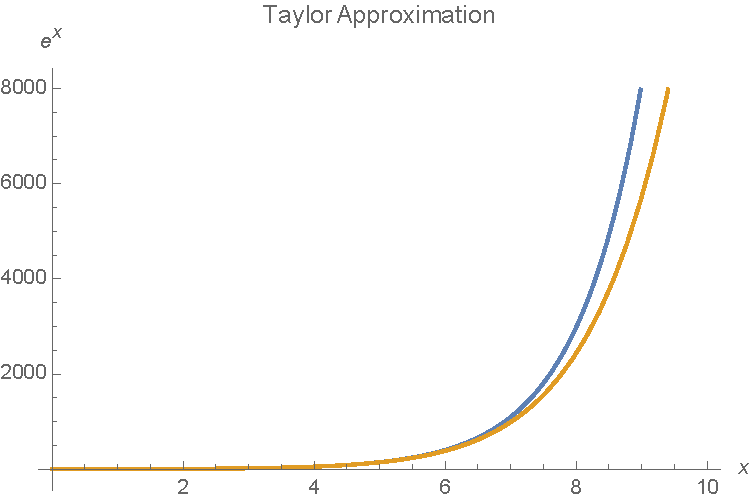
\includegraphics[width=0.65\textwidth]{Exp.pdf}
\caption{Comparing $e^x$ with its Taylor approximation centered at zero.}\label{exp}
\end{centering}
\end{figure}

\begin{figure}[bth]
\begin{centering}
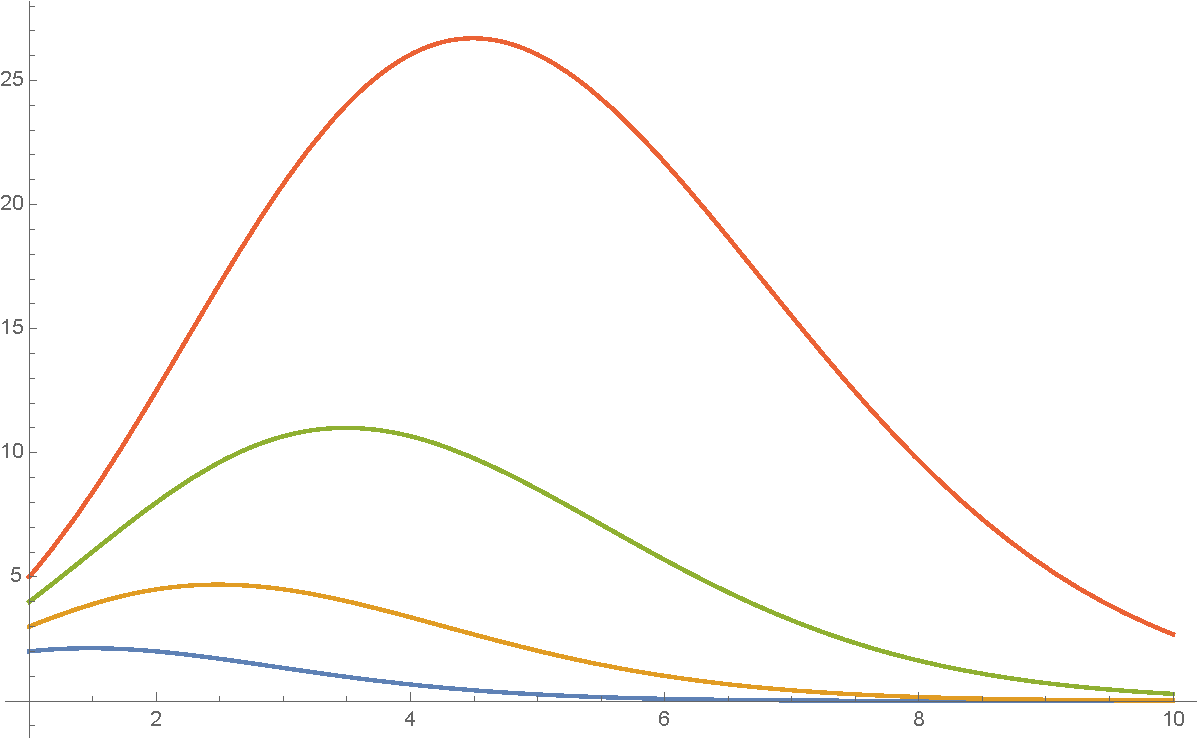
\includegraphics[width=0.75\textwidth]{Growth}
\caption{Comparing $\dfrac{x^k}{k!}$ for $x=2,3,4,5$.}\label{growth}
\end{centering}
\end{figure}

If we are na\"ive about computing the terms of the series we can
quickly get into trouble --- the values of $k!$ get large \emph{very quickly}.
We can do better if we observe that:
$$
\frac{x^k}{k!} = \frac{x^{k-1}}{(k-1)!} \times \frac{x}{k} .
$$


At first, that looks like a recursive definition (and in fact, you
could write it that way, but it would be wasteful). As we progress
through the computation, assume that we know the previous result.
We then just have to compute the next term and multiply it by the
previous term.  At each step we just need to compute $\frac{x}{k}$,
starting with $k = 0!$ (remember $0! = 1$) and multiply it by the previous value and
add it into the total. It turns into a simple \texttt{for} or
\texttt{while} loop.

Conceptually, what you need to think about is:
\begin{codelisting}{}
  new = previous * current;
  previous = current;
\end{codelisting}

We can use an $\epsilon$ (epsilon) to halt the computation since
$|x^k| < k!$ for a sufficiently large $k$.  Consider Figure \ref{growth}:
briefly, $x^k$ dominates but is quickly overwhelmed by $k!$ and so
the ratio rapidly approaches zero.
\textcolor{red}{You should set $\epsilon = 10^{-14}$ for this assignment.} \\


\subsection{Log}

To compute $\log$, you will use Newton's method, also called the Newton-Raphson
method. It is an iterative algorithm to approximate roots of real-valued
functions, \textit{i.e.}\xspace, solving $f(x) = 0$. Each iteration of Newton's
method produces successively better approximations.
\[
  x_{k+1} = x_k - \frac{f(x_k)}{f'(x_k)}
\]

For example, consider computing \emph{square roots} with Newton's method. That
is, in order to solve for some $\sqrt{y}$, we are searching for a positive $x$
such that $x^2 = y$. We can express this as finding the root of $f(x) = x^2 -
y$, giving us:
\[
  x_{k+1} = \frac{1}{2}(x_k + \frac{y}{x_k}).
\]

Each guess $x_{k+1}$ gives a successive improvement over the previous guess
$x_k$. The following is an example that implements Newton's method of computing
square roots that doesn't conflict with \texttt{sqrt()} found in
\texttt{<math.h>}. Note that the function is named \texttt{Sqrt()}. It begins
with an initial guess $x_0 = 1.0$ that it uses to compute better approximations.
The square root is said to be calculated once the value converges,
\textit{i.e.}\xspace the difference between consecutive approximations is small.

\begin{codelisting}{Computing $\sqrt{x}$ using Newton's method.}
#define EPSILON 1e-9

static inline double Abs(double x) {
  return x < 0 ? -x : x;
}

double Sqrt(double y) {
  double x_n = 1.0;
  double old = 0.0;
  while (Abs(x_n - old) > EPSILON) {
    old = x_n;
    x_n = 0.5 * (x_n + y / x_n);
  }
  return x_n;
}
\end{codelisting}

Your function \texttt{Log()} should behave the same as \texttt{log()} from
\texttt{<math.h>}: compute $\ln(x)$. The procedure is very much the same as it
was for the square root example, the main difference being that $f(x) = y -
e^x$, since $e^x$ is the inverse of $\ln$, \textit{i.e.} $\ln(e^x) = x$. Another
key difference is the value converges when $e^{x_{i}} - y$ is small, where
$x_{i}$ is initially $1.0$ and is used to compute better approximations. In
order to implement this function, you will have to use your \texttt{Exp()}
function. Using the \texttt{exp()} function from \texttt{<math.h>} is strictly
prohibited.

\section{Command-line Options}
\epigraphwidth=0.75\textwidth
\epigraph{\emph{GUIs tend to impose a large overhead on every single piece of
    software, even the smallest, and this overhead completely changes the
    programming environment. Small utility programs are no longer worth writing.
    Their functions, instead, tend to get swallowed up into omnibus software
packages.}}{---Neal Stephenson, \emph{In the Beginning\ldots Was the Command
Line}}

Your test harness will determine which implemented functions to run through the
use of \emph{command-line options}. In most \textbf{C} programs, the
\texttt{main()} function has two parameters: \texttt{int argc} and \texttt{char
**argv}. A command, such as \texttt{./hello arg1 arg2}, is split into an array
of strings referred to as arguments. The parameter \texttt{argv} is this array
of strings. The parameter \texttt{argc} serves as the argument counter, the
value in which is the number of arguments supplied. Try this code, and make sure
that you understand it:

\begin{codelisting}{Trying out command-line arguments.}
#include <stdio.h>

int main(int argc, char **argv) {
    for (int i = 0; i < argc; i += 1) {
        printf("argv[%d] = %s\n", i, argv[i]);
    }
    return 0;
}
\end{codelisting}

A command-line option is an argument, usually prefixed with a hyphen,
that modifies the behavior of a command or program. They are typically parsed
using the \texttt{getopt()} function. \emph{Do not} attempt to parse the command-line
arguments yourself. Instead, use the \textit{getopt()} function. Command-line options
must be defined in order for \texttt{getopt()} to parse them. These options are defined
in a string, where each character in the string corresponds to an option character
that can be specified on the on the command-line. Upon running the executable,
\texttt{getopt()} scans through the command-line arguments, checking for option
characters.

\begin{codelisting}{Parsing options with \texttt{getopt()}.}
#include <stdio.h>
#include <unistd.h> // For getopt().

#define OPTIONS "pi:"

int main(int argc, char **argv) {
    int opt = 0;
    while ((opt = getopt(argc, argv, OPTIONS)) != -1) {
        switch (opt) {
        case 'p':
            printf("-p option.\n");
            break;
        case 'i':
            printf("-i option: %s is parameter.\n", optarg);
            break;
        }
    }
    return 0;
}
\end{codelisting}

This example program supports two command-line options, `\texttt{p}' and
`\texttt{i}'. Note that the option character `\texttt{i}' in the defined option
string \texttt{OPTIONS} has a colon following it. The colon signifies that, when
the `\texttt{i}' option is enabled on the command-line using `\texttt{-i}',
\texttt{getopt()} is looking for an parameter to be supplied following it. An
error is thrown by \texttt{getopt()} if an argument for a flag requiring one is
not supplied.


\section{Deliverables}

\epigraphwidth=0.6\textwidth
\epigraph{\emph{Thinking doesn't guarantee that we won't make mistakes. But
not thinking guarantees that we will.}}{---Leslie Lamport}

\noindent You will need to turn in:
\begin{enumerate}
  \item \texttt{mathlib.h}: You will be supplied this file and \textcolor{red}{you \emph{are not} allowed
    to modify it}. The function prototypes for the math functions you are
    required to implement are as follows:
    \begin{itemize}
      \item \texttt{double Sin(double x);}
      \item \texttt{double Cos(double x);}
      \item \texttt{double Tan(double x);}
      \item \texttt{double Exp(double x);}
      \item \texttt{double Log(double x);}
    \end{itemize}

  \item \texttt{mathlib.c}: This file will contain your math function
    implementations, as prototyped in \texttt{mathlib.h}. Your functions
    \emph{must not} print or have any side effects.

  \item \texttt{mathlib-test.c}: This file will contain the \texttt{main()}
    program and acts as a test harness for your math library. The code to parse
    command-line options and print out the results of testing your math
    functions belong here. The \texttt{getopt()} options you \emph{must}
    support are:
    \begin{itemize}
      \item \texttt{-a}: to run all tests.
      \item \texttt{-s}: to run $\sin$ tests.
      \item \texttt{-c}: to run $\cos$ tests.
      \item \texttt{-t}: to run $\tan$ tests.
      \item \texttt{-e}: to run $e^x$ tests.
      \item \texttt{-l}: to run $\log$ tests.
    \end{itemize}
    Note that these options are \emph{not} mutually exclusive. You should be
    able to support any combination of these options. Each function is tested at
    most once. Specifying all tests to be run and a specific test does not
    result in that test running twice (\textit{e.g.}\xspace \texttt{./mathlib-test -a -s}). The
    output for each function must match the format shown in Figures~\ref{sine}
    and~\ref{cosine}. Your compiled program must be called
    \texttt{mathlib-test}. To aid you with the print formatting, the print
    statement is given as follows:

    \begin{codelisting}{}
printf(" %7.4lf % 16.8lf % 16.8lf % 16.10lf\n", ...);
    \end{codelisting}

    The spaces in the print format statement are \emph{intentional} and account for
    negative (but not positive) signs.

  \item \texttt{Makefile}: This is a file that will allow the grader to type
    \texttt{make} to compile your program. Running \texttt{make} or \texttt{make
    all} must build your \texttt{mathlib-test} program. Running \texttt{make clean}
    must remove any compiler-generated files.

  \item \texttt{README.md}: This must be in \emph{Markdown}. This must describe
    how to build and run your program and list the command-line options it
    accepts and what they do.

  \item \texttt{DESIGN.pdf}: This \emph{must} be a PDF\@. The design document
    should contain answers to the pre-lab questions. It should also describe the
    purpose of your program and communicate the overall design of the program
    with enough detail such that a sufficiently knowledgeable programmer would
    be able to replicate your implementation. \textcolor{red}{This does not
    mean copying your entire program in verbatim.} You should instead describe
    how your program works with supporting pseudocode.
    \textcolor{red}{\textbf{C} code is \textbf{not} considered pseudocode.} You
    \emph{must} push \texttt{DESIGN.pdf} before you push \textcolor{red}{\emph{any}}
    code.

  \item \texttt{WRITEUP.pdf}: This \emph{must} be a PDF\@. \texttt{WRITEUP.pdf}
    should contain a discussion of the results for your tests. This means
    analyzing the differences in the output of your implementations versus those
    in the \texttt{<math.h>} library. Include possible reasons for the differences
    between your implementation and the standard library's. Graphs can be
    especially useful in showing the differences and backing up your arguments.
\end{enumerate}


\section{Submission}

\epigraph{\emph{We in science are spoiled by the success of mathematics.
Mathematics is the study of problems so simple that they have good
solutions.}}{---Whitfield Diffie}

To submit your assignment, refer back to \texttt{asgn0} for the steps on how to
submit your assignment through \texttt{git}. Remember: \emph{add, commit,} and
\emph{push}!

\textcolor{red}{Your assignment is turned in \emph{only} after you have pushed.
If you forget to push, you have not turned in your assignment and you will get a
\emph{zero}. ``I forgot to push'' is not a valid excuse. It is \emph{highly}
recommended to commit and push your changes \emph{often}.}


\section{Supplemental Readings}

\epigraph{\emph{The more that you read, the more things you will know. The
more that you learn, the more places you'll go.}}{---Dr.\ Seuss}\noindent

\begin{itemize}
  \item \textit{The C Programming Language} by Kernighan \& Ritchie
  \begin{itemize}
    \item Chapter 3 \S 3.4-3.7
    \item Chapter 4 \S 4.1 \& 4.2 \& 4.5
    \item Chapter 7 \S 7.2
    \item Appendix B \S B4
  \end{itemize}

  \item \textit{The Kollected Kode Vicious } by George V. Neville-Neil
  \begin{itemize}
      \item Chapter 2 \S 2.6
  \end{itemize}
\end{itemize}

\end{document}

